\only<presentation>{
\begin{frame}[label=uebersicht]{Kursus / Übersicht}
  \textbf{19.01.2018 : Datenbanktechnologien II: BigData}
  \begin{itemize}
    \item kurze Wiederholung --- wo stehen wir?
    \item Exkurs: Das DOM für automatisiertes Testen von WebApplikationen verwenden
    \item Klärung verschiedener Begriffe und Buzzwords
    \item Anwendungsszenarien von Big Data, Anwendung in der ETH--Bibliothek
    \item In Medias Res: DataScience am Bsp. Logfiles und Benutzerdaten, BigData am Bsp. OAI--Server
  \end{itemize}
\end{frame}
}


\subsection{Exkurs: Das DOM für automatisiertes Testen von WebApplikationen verwenden}
\only<article>{
  Bei jedem Update einer Software stellt sich uns das Problem, dass wir überprüfen wollen, ob sie noch so funktioniert, wie bestellt. So testen wir beispielsweise bei unserem Discovery Portal, ob sich die Indexierung verändert hat, oder ob der Date--Slider noch funktioniert. Aber warum sollten wir das manuell machen?

  Nachdem wir das DOM verwendet haben, um vielfältige Funktionen auf einer Webseite zu realisieren, können wir es auch benutzen, um diese Funktionen automatisch vom Computer testen zu lassen. Das wollen wir uns im Folgenden mal anschauen.

  Unser Ziel ist es, das ein Computer die Webseite wie ein normaler Benutzer aufruft, die Services nutzt und dabei testet, ob alles wie gewünscht funktioniert.

  Da taucht übrigens die erste Schwierigkeit auf: Was ist ,,wie gewünscht''? Fragen wir drei Personen nach einem Feature, bekommen wir mindestens vier verschiedene Antworten.

  Indem man sich nun über die zu testenden Funktionen abspricht, deckt man quasi nebenbei derartige Missverständnisse schnell auf. Mehr dazu in meinem Artikel \href{http://dx.doi.org/10.1515/abitech-2017-0025}{,,Automatisiertes Testen von Webapplikationen'' [Link]}.

  Was kann der Computer nun tun?

  Beispielsweise lassen sich Elemente einer Webseite mit Skriptsprachen auf den korrekten Inhalt prüfen. Wir hatten das in dem Beispiel schon gesehen, in dem es darum ging, eine Tabellenzeile ein-- bzw. auszublenden.
  }

\begin{frame}[fragile]{den Inhalt eines Elements einer Webseite abfragen}
  \fontencoding{T1}\selectfont
  \begin{lstlisting}
<script type="text/javascript">
  function einausblenden(id) {
    var meinElement = document.getElementById(id);
    if (meinElement.style.display === "none") {
      meinElement.style.display = "table-row";
    } else {
      meinElement.style.display = "none";
    }
  }
</script>
  \end{lstlisting}
\end{frame}

\only<article>{
  Mittels Ruby und den FrameWorks ,,Cucumber'' und ,,Capybara'' testen wir nach jedem Update von Primo, ob die Features noch so funktionieren, wir wir es geplant haben:
}

\begin{frame}[<+->]{automatisierte Tests von Primo}
  \begin{itemize}
    \item Wir prüfen nach einem Update, ob sich die Suchalgorithmen verändert haben, indem wir die Trefferzahl zwischen den beiden Systemen mit identischem Datenstand vergleichen.
    \item Der Date--Slider hat in der Vergangenheit Probleme gemacht. Wir checken, ob er plausible Ranges liefert.
    \item Wir testen, ob nicht--lateinische Schriftzeichen gefunden werden.
    \item \ldots
  \end{itemize}
\end{frame}

\only<article>{
  Das Gute an dem verwendeten FameWork ist, dass die Anforderungen nahezu natürlichsprachig formuliert werden. So stellen wir sicher, dass IT und ,,normale'' Menschen vom Gleichen sprechen.
}

\begin{frame}[fragile]{eine Anforderung in Gherkin formuliert}
  \fontencoding{T1}\selectfont
  \begin{lstlisting}
Szenario: Eine Suche ergibt auf den beiden Prod Systemen eine ähnliche Anzahl Treffer
    Wenn ich die Seite "http://terza-prod1-fe41.ethz.ch/primo-explore/search?vid=DADS&sortby=rank&lang=de_DE" aufrufe,
    Und ich in den Suchschlitz "Wald" eingebe,
    Und die Anzahl der Treffer nehme
    Und dann die Seite "http://terza-prod2-fe41.ethz.ch/primo-explore/search?vid=DADS&sortby=rank&lang=de_DE" aufrufe,
    Wenn ich in den Suchschlitz den Suchbegriff "Wald" eingebe,
    Und dort die Anzahl der Treffer nehme
    Dann sollten die Treffermengen ähnlich, d.h. die Abweichung unter 1\%, sein.
  \end{lstlisting}
\end{frame}

\only<article>{
  Schauen wir uns dazu eine Seite im UI von Primo an. Wir wollen in den Suchschlitz das Wort ,,Wald'' eingeben. 
  \pagebreak
}

\begin{frame}{Der Suchschlitz im alten UI}
  \begin{center}
    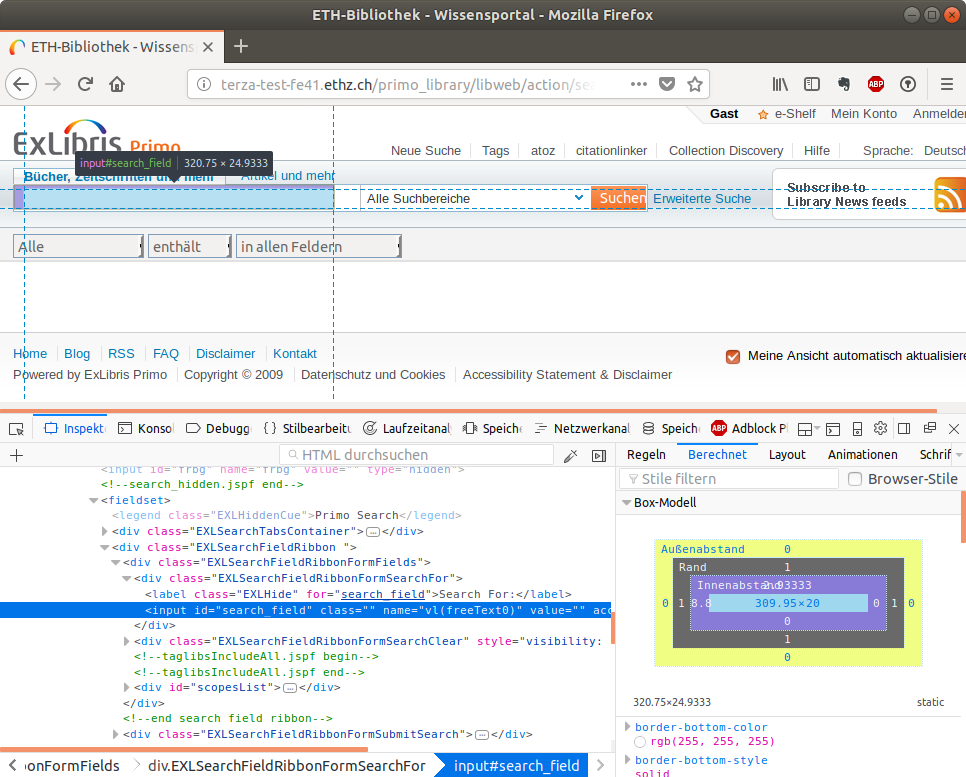
\includegraphics[width=1\textwidth]{pics/old-ui-searchbar}
  \end{center}
\end{frame}

\begin{frame}[fragile]{der Quellcode des Suchschlitzes (altes UI)}
  \fontencoding{T1}\selectfont
  \begin{lstlisting}[language=html]
<input name="vl(freeText0)" class="" value="" id="search_field" accesskey="s" type="text">
  \end{lstlisting}
\end{frame}

\only<article>{
  Den Suchschlitz können wir also ansteuern, indem wir im DOM nach der ID ,,search\_field'' suchen.

  Ein Problem ist, dass sich IDs nach Updates ändern können.
  \pagebreak
}

\begin{frame}{Der Suchschlitz im neuen UI}
  \begin{center}
    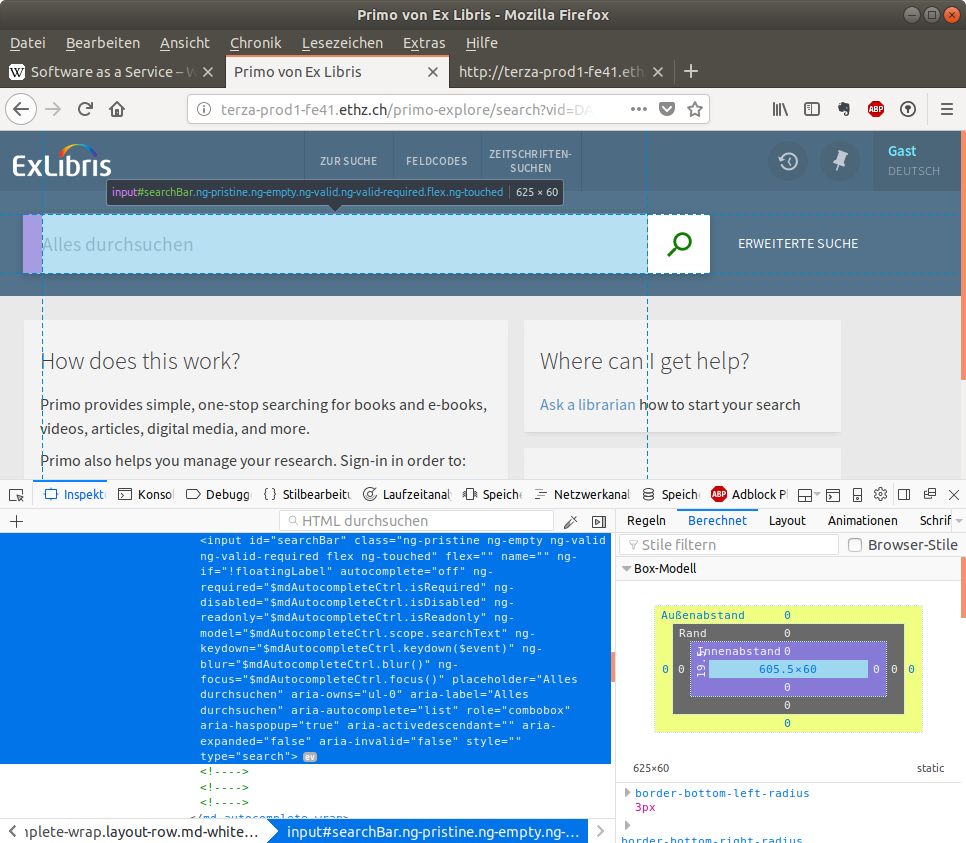
\includegraphics[width=1\textwidth]{pics/pnui-searchbar}
  \end{center}
\end{frame}

\begin{frame}[fragile]{der Quellcode des Suchschlitzes (neues UI)}
  \fontencoding{T1}\selectfont
  \begin{lstlisting}[language=html]
<input flex="" id="searchBar" name="" ng-if="!floatingLabel" autocomplete="off" ng-required="$mdAutocompleteCtrl.isRequired" ng-disabled="$mdAutocompleteCtrl.isDisabled" ng-readonly="$mdAutocompleteCtrl.isReadonly" ng-model="$mdAutocompleteCtrl.scope.searchText" ng-keydown="$mdAutocompleteCtrl.keydown($event)" ng-blur="$mdAutocompleteCtrl.blur()" ng-focus="$mdAutocompleteCtrl.focus()" placeholder="Alles durchsuchen" aria-owns="ul-0" aria-label="Alles durchsuchen" aria-autocomplete="list" role="combobox" aria-haspopup="true" aria-activedescendant="" aria-expanded="false" class="ng-pristine ng-empty ng-valid ng-valid-required flex ng-touched" aria-invalid="false" style="" type="search">
  \end{lstlisting}
\end{frame}

\only<article>{
  Die ID heisst nun ,,searchBar''. Die Tests müssen darauf angepasst werden. Im nächsten Schritt verwenden wir nun die ID, um ein Suchwort in den Suchschlitz zu schreiben.
}

\begin{frame}[fragile]{Ruby--Snippet, um ,,Wald'' in den Suchschlitz zu schreiben}
  \fontencoding{T1}\selectfont
  \begin{lstlisting}[language=ruby]
Wenn(/^ich in den Suchschlitz "(^*)" eingebe,\$/) do |q|
  fill_in('#searchBar', with: q)
  find(".button-confirm").send_keys(:enter)
end
  \end{lstlisting}
\end{frame}

\only<article>{
  Mit dieser Technik lassen sich alle Elemente auf einer Webseite ansteuern, auslesen und bedienen. So lassen sich komplexe Tests schreiben und dann automatisch vom Computer durchführen.
}

\begin{frame}{Der Testablauf auf der Kommandozeile}
  \begin{center}
    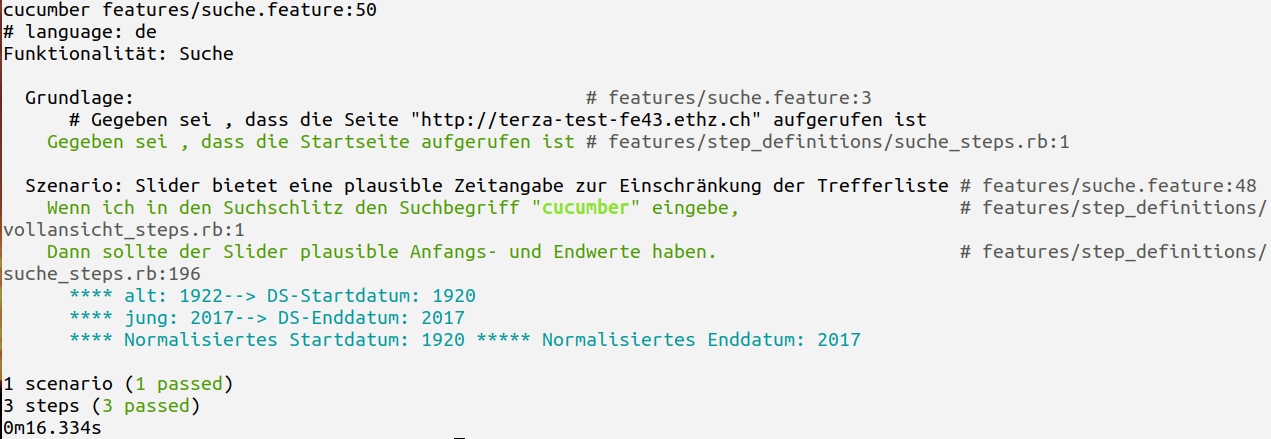
\includegraphics[width=1\textwidth]{pics/cucumber-test}
  \end{center}
  \only<presentation>{Die Ausgabe gibt es auch als \href{http://allegra.ethz.ch/tests/2017/04/20170416.html}{Webseite}.}
\end{frame}

\only<article>{
  \pagebreak

  und als Webseite: 
  
  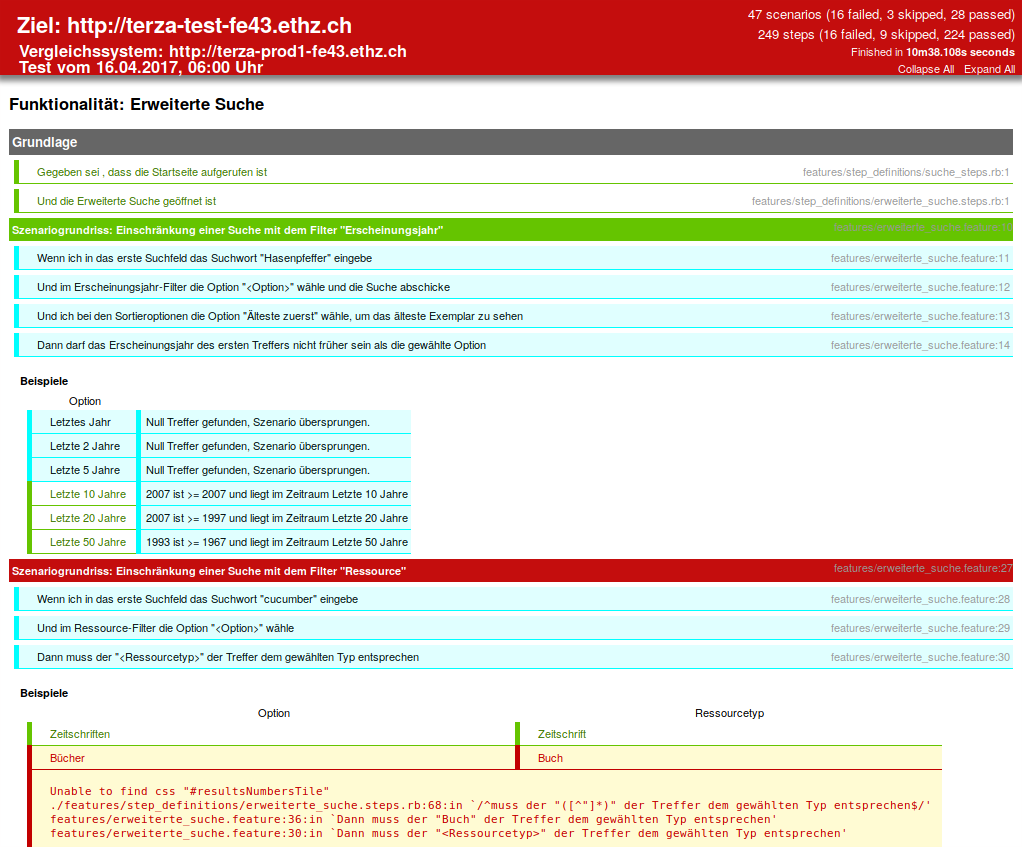
\includegraphics[width=1\textwidth]{pics/Testausgabe_webseite}

  Da man die Ausgabe der Test--Ergebnisse auch als Datei --- beispielsweise als html--Datei --- abspeichern kann, bietet es sich an, diese Tests regelmässig auf einem Server auszuführen und die Ergebnisse als Webseiten den Productownern zur Verfügung zu stellen.
}

\section{Datenbanktechnologien II: BigData}
\subsection{Klärung verschiedener Begriffe und Buzzwords}

\only<article>{
  Beginnen wir mit der berühmten Cloud. Wer heute etwas in der IT zu entscheiden hat, geht in die Cloud. Die Cloud ist die Lösung für alle IT--Probleme!

  Oder?

  Die Cloud bietet für viele Anwendungszenarien praktische Lösungen. 
  }


\begin{frame}[<+->]{Dienstleistungen in der Cloud}
  Wir erinnern uns:
  \begin{itemize}
    \item SaaS
    \item IaaS
    \item PaaS
  \end{itemize}
\end{frame}


\only<article>{
  Ein Problem ist, dass die Services stark standardisiert sind. Ein System, in dem alle vollkommen unabhängig von den eigenen Anforderungen dieselben Services beziehen, ist nicht erfolgreich. So gab es beispielsweise in der DDR für alle nur Trabbis, obwohl sicher nicht alle das gleiche Auto fahren wollten.

  Ein anderes ist die Frage, welche Daten herausgegeben werden. Die Free Software Foundation formuliert es sehr klar:
  }

\begin{frame}
  \begin{quote}
    It's not the Cloud, it's just other people's computers.
  \end{quote}
\end{frame}


\only<article>{
  Nochmal deutlich: Cloud bedeutet, dass uns jemand einen Teil der Arbeit abnimmt und dafür unsere Daten nutzt! So bietet Google hervorragende Services kostenlos an --- im Tausch für unsere Daten.

  Im Falle von Bibliothekssoftware bekommt der Anbieter zusätzlich zu unseren Daten noch eine Menge Geld.

  Um nun entsprechende Systeme aufzubauen, mit denen man derartige Dienstleistungen anbieten kann, benötigt man besondere Techniken mit denen man sehr grosse Datenmengen verarbeiten und speichern kann. 

  So kommen wir zu BigData.
  }

\subsection{Anwendungsszenarien von Big Data, Anwendung in der ETH--Bibliothek}


\begin{frame}{}
  \begin{center}
    
\includegraphics[height=0.8\textheight]{pics/vvv}
  \end{center}
\end{frame}

\begin{frame}{eine Definition}
  Der aus dem englischen Sprachraum stammende Begriff Big Data [ˈbɪɡ ˈdeɪtə] (von englisch big ‚groß‘ und data ‚Daten‘) bezeichnet Datenmengen, welche
  \begin{itemize}
    \item zu groß,
    \item zu komplex,
    \item zu schnelllebig
    \item zu schwach strukturiert
  \end{itemize}
  sind, um sie mit manuellen und herkömmlichen Methoden der Datenverarbeitung auszuwerten.
  \bigskip

  \footnotesize{[Seite „Big Data“. In: Wikipedia, Die freie Enzyklopädie. Bearbeitungsstand: 21. Oktober 2017, 06:34 UTC. URL: https://de.wikipedia.org/w/index.php?title=Big_Data&oldid=170175574 (Abgerufen: 26. Oktober 2017, 14:31 UTC)]}
\end{frame}

\begin{frame}{}
  \begin{center}
    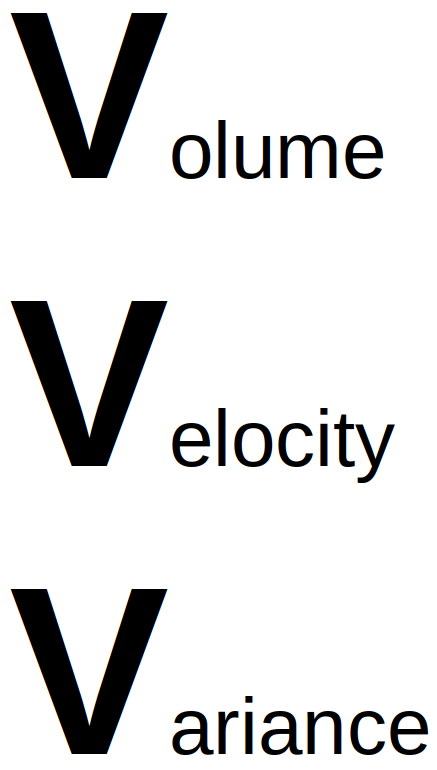
\includegraphics[height=0.8\textheight]{pics/vdescription}
  \end{center}
\end{frame}

\begin{frame}{Was ist nun BigData?}
  \fbox{\parbox[c][0.5\textheight][t]{0.3\linewidth}{
    \textbf{DataScience}

    Wissensgewinnung
    \begin{itemize}
      \item Sichtung
      \item Umwandlung
      \item Analyse
      \item Visualisierung
    \end{itemize}
  }}
  \fbox{\parbox[c][0.5\textheight][t]{0.3\linewidth}{
    \textbf{BigData}

    Datenhaltung
    \begin{itemize}
      \item Speicherung
      \item Sicherung
      \item Abfrage
    \end{itemize}
  }}
  \fbox{\parbox[c][0.5\textheight][t]{0.3\linewidth}{
    \textbf{MachineLearning}

    KI
    \begin{itemize}
      \item Training
      \item Klassifizierung
      \item Vorhersage
    \end{itemize}
  }}
\end{frame}

\only<article>{
  Umgangssprachlich wird BigData für alle drei Themen genutzt. So bedeutet die innovative Idee ,,Lasst uns mal BigData machen'' in der Regel nicht, uns eine neue Datenbank zuzulegen.

  Um uns den Möglichkeiten in Bibliotheken weiter zu nähern, fangen wir mit einer Selbsteinschätzung an.
}

\only<presentation>{
\begin{frame}{}
    Und bei uns? 10 Millionen Datensätze sind doch 'ne ganze Menge\ldots
\end{frame}
}

\pagebreak

\begin{frame}{Datenmengen an der ETH--Bibliothek}
  \begin{itemize}
    \item Bildarchiv Online: ca. 600‘000 Datensätze
    \item Aleph: ca. 7,9 Millionen Datensätze
    \item Primo: ca. 10,1 Millionen Datensätze
  \end{itemize}
\end{frame}

\only<article>{
  Obwohl 10,1 Millionen Datensätze in einem Bibliothekskatalog schon eine ganze Menge sind, kommt es bei Weitem nicht an die Mengen heran, die üblicherweise mit BigData bezeichnet werden. 
}

\begin{frame}{ein frustrierender Vergleich:}
    Ein Beispiel für Datensatzzahlen im BigData--Bereich sind die ca. 15 Milliarden Tweets  die über Twitter in einem Monat versendet werden.
\end{frame}


\only<presentation>{
\begin{frame}{}
  \begin{center}
    Und wie schnell verändern sich die Daten?
  \end{center}
\end{frame}
}

\only<article>{
  Auch sind die Datenzuwächse und --veränderungen bei uns nicht mit denen im BigData--Business vergleichbar.

  Hier ein paar Zahlen aus dem Web: 
}

\begin{frame}\only<presentation>{{Velocity im WWW}}
  \begin{center}
    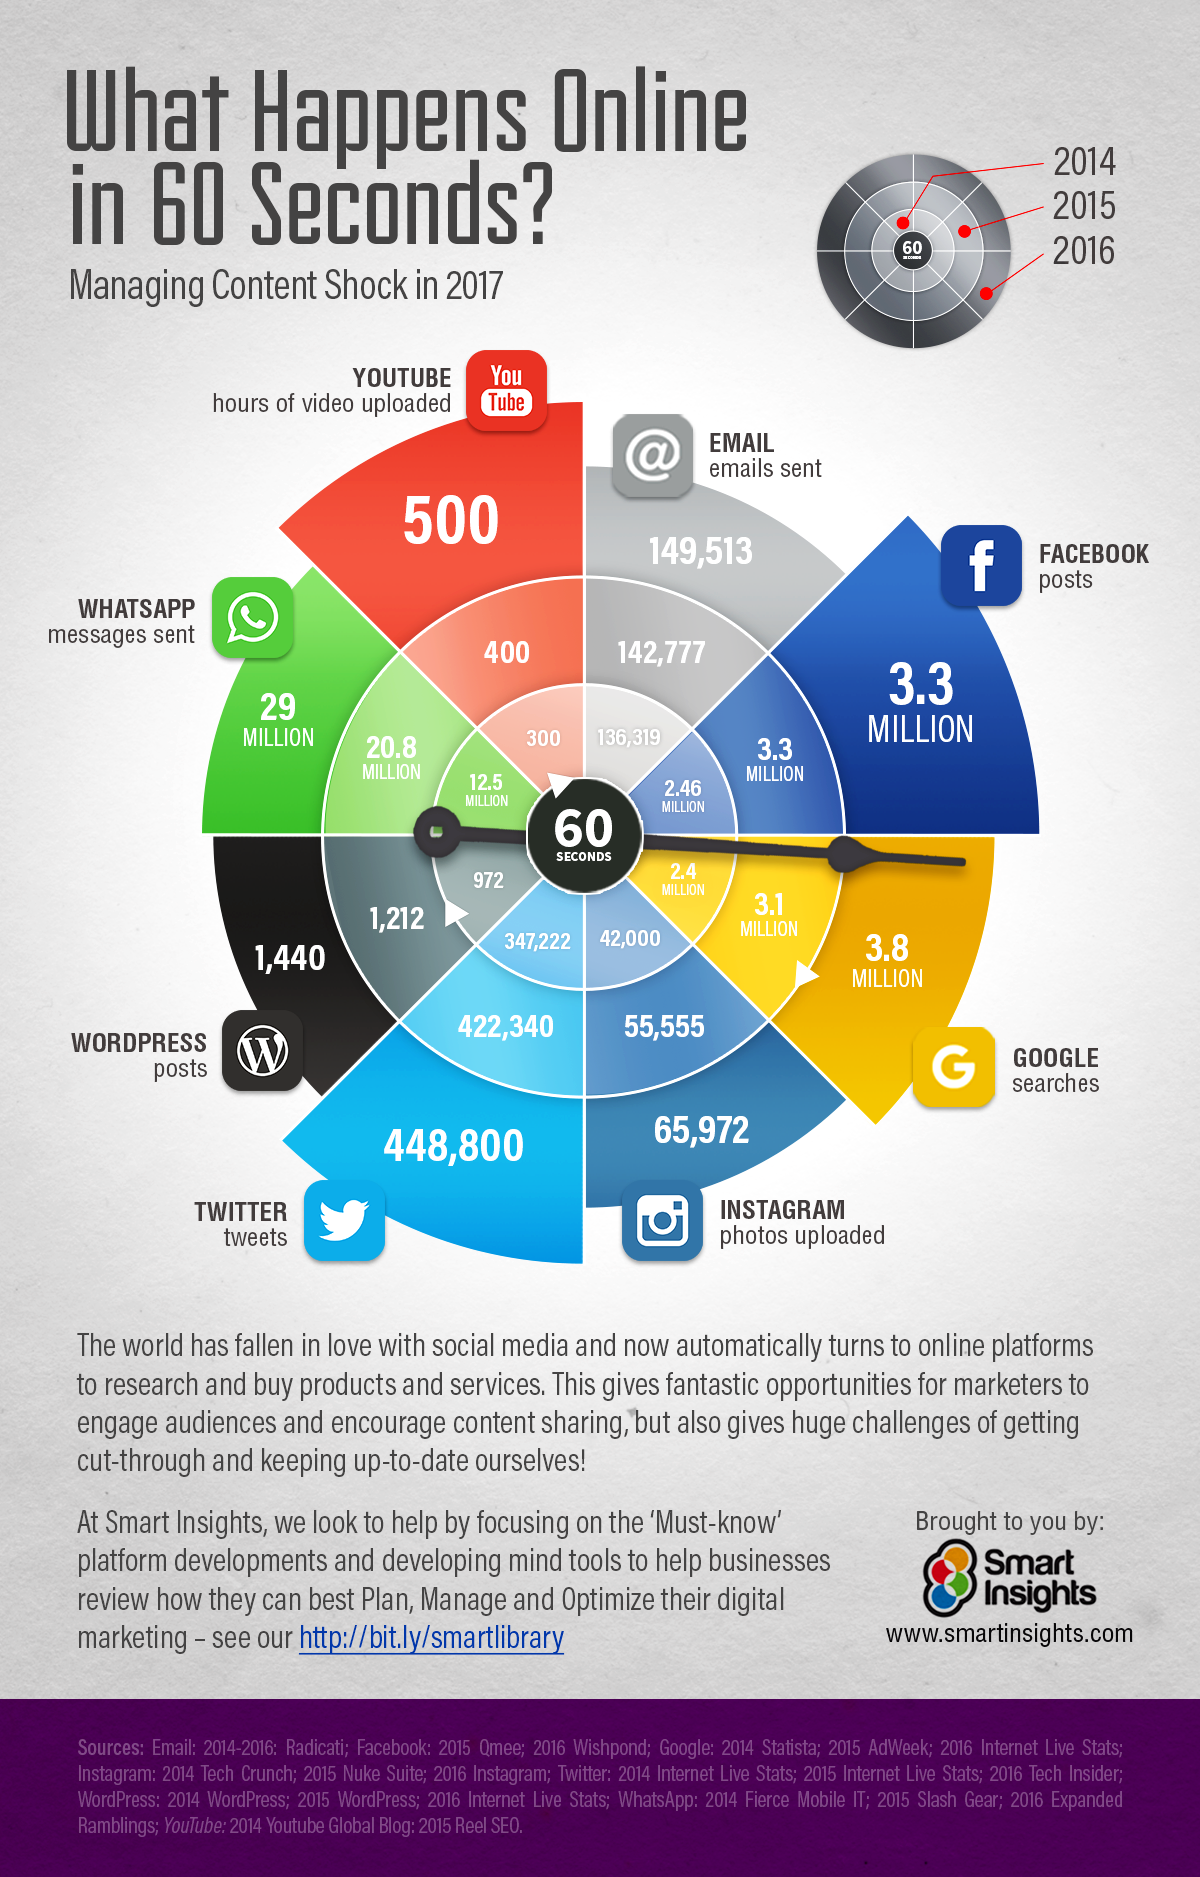
\includegraphics[height=1\textheight]{pics/velocity}
  \end{center}
\end{frame}

\only<presentation>{
\begin{frame}{}
  \begin{center}
    Und die Varianz?
  \end{center}
\end{frame}
}

\only<article>{
  Auch die Varianz ist bei unseren Metadaten --- hoffentlich --- nicht gross. Im Gegenteil, unsere Daten sind nach klaren Regeln erfasst und idealerweise über Systemgrenzen austauschbar.
}

\begin{frame}[fragile]{Varianz}
  \framesubtitle{ein Buch}
  \fontencoding{T1}\selectfont
  \begin{lstlisting}[language=xml]
<recordid>ebi01_prod010616366</recordid>
<type>book</type>
<title>Sophocles: four tragedies</title>
<creator>Sophocles, v497-v407</creator>
<creator>Oliver Taplin, 1943-</creator>
<edition>First edition</edition>
<publisher>Oxford, United Kingdom : Oxford University Press</publisher>
<creationdate>2015</creationdate>
<subject>Sophocles -- Translations into English</subject>
<subject>Oedipus, Greek mythological figure – Drama</subject>
  \end{lstlisting}
\end{frame}

\begin{frame}[fragile]{Varianz}
  \framesubtitle{ein Bild}
  \fontencoding{T1}\selectfont
  \begin{lstlisting}[language=xml]
<recordid>ebi01_prod010103021</recordid>
<type>image</type>
<title>[Aias und Kassandra]</title>
<creator>Heinrich Meyer, 1760-1832</creator>
<creator>Johann Heinrich Lips, 1758-1817</creator>
<publisher>[Weimar]</publisher>
<creationdate>[1794]</creationdate>
<format>1 Druckgraphik : Aquatinta und Radierung in Schwarz und Braunrot ; Bild 18,5 x 23,1 cm, Blatt 23,4 x 32,2 cm</format>
<identifier><b>DOI: </b>10.3931/e-rara-37966 ; $$CBIBL$$VJoachim Kruse: Johann Heinrich Lips 1758-1817, Coburg 1989, S. 220 ; $$CBIBL$$VErschienen in: Heinrich Meyer/Carl August Böttiger (Hg.): Über den Raub der Cassandra auf einem alten Gefässe von gebrannter Erde, Weimar 1794, S. 93</identifier>
<subject>Kassandra, Fiktive Gestalt</subject>
<subject>Athena, Göttin</subject>
  \end{lstlisting}
\end{frame}

\begin{frame}{ergo}
  \begin{center}
    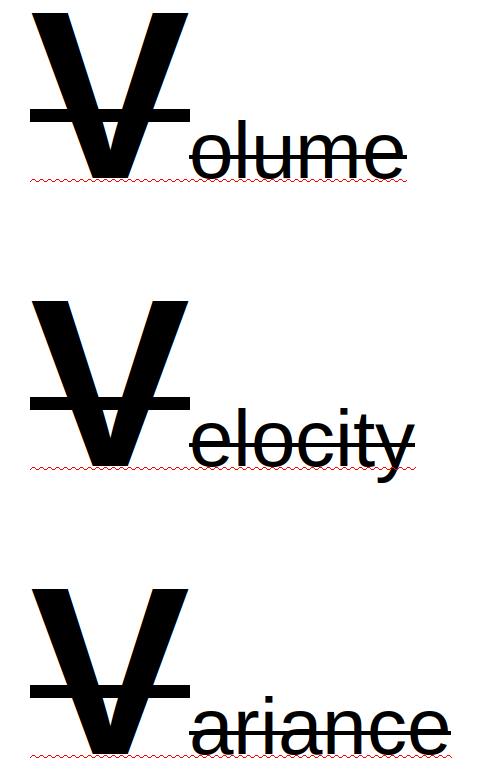
\includegraphics[height=0.8\textheight]{pics/nix_v}
  \end{center}
\end{frame}

\begin{frame}{BigData ohne Big Data?}
    Wir haben so wenige, so gut strukturierte Daten, dass wir kein Einsatzszenario für BigData entwickeln können, bei dem die Kosten/Nutzen-Rechnung stimmt.
\end{frame}

\only<article>{
  Auch für eine sinnvolle Anwendung von MachineLearning reichen unsere Daten kaum aus. Microsoft Research hat das gut verdeutlicht. Um angemessen akkurate Aussagen treffen zu können, benötigt man mehr als 50 Millionen Datensätze.
}

\begin{frame}[fragile]{machine learning}
  \fontencoding{T1}\selectfont
  \begin{columns}[t,onlytextwidth]
    \begin{column}{0.5\textwidth}
      \begin{center}
        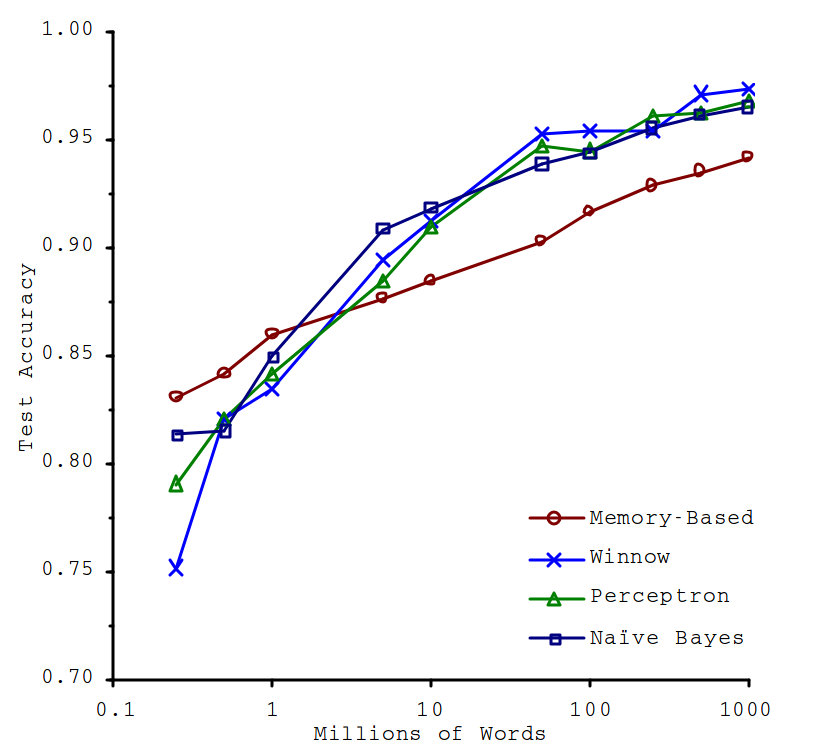
\includegraphics[width=1\textwidth]{pics/wann_effektiv}
      \end{center}
    \end{column}
    \begin{column}{0.5\textwidth}
      \\
      \medskip

      Eine Studie von Microsoft Research kommt bei einem Vergleich verschiedener Klassifizierungsalgorithmen zu dem Ergebnis, das die Tests erst ab ca. 50 Millionen Datensätzen eine befriedigende Genauigkeit aufweisen.
      \bigskip
      
      \footnotesize{[Michele Banko and Eric Brill, Microsoft Research: Scaling to Very Very Large Corpora for Natural Language Disambiguation]}
    \end{column}
  \end{columns}
\end{frame}

\subsection{In Medias Res: DataScience am Bsp. Logfiles und
Benutzerdaten, BigData am Bsp. OAI--Server}
\only<article>{
  Allerdings können wir einzelne Technologien aus dem BigData--Bereich durchaus gewinnbringend einsetzen. So lassen sich beispielsweise grosse Mengen an Log--Daten mit modernen DataScience--Methoden gut sichten und für erste Auswertungen nutzen.

  Mit der Auswertung von Logfiles lassen sich Aussagen zum Nutzerverhalten treffen. Dabei kommen zunächst Methoden der IT zum Einsatz:
}

\begin{frame}{anonymisierte Logdaten aus dem Discovery--Portal}
  \framesubtitle{1. Auszug relevanter Zeilen mit klassischen Methoden}
  So werden aus insgesamt 158'203'686 Zeilen aus 617 Logfiles 6'405'616 relevante Zeilen extrahiert:
  \begin{center}
    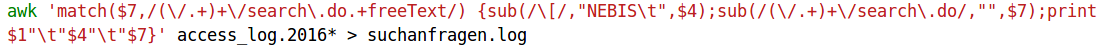
\includegraphics[width=1\textwidth]{pics/bsp-awk}
  \end{center}
\end{frame}

\begin{frame}{anonymisierte Logdaten aus dem Discovery--Portal}
  \framesubtitle{2. Visualisierung mit DataScience--Methoden}
  Mit der Sprache Python werden die Daten in ein Dataframe geladen und können so in beliebigen Ausschnitten gesichtet werden, um anhand von Stichproben die weiteren Bearbeitungsschritte festzulegen\ldots
  \begin{center}
    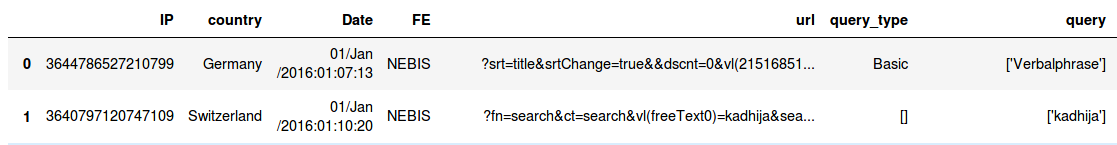
\includegraphics[width=1\textwidth]{pics/Ausschnitt_Dataframe}
  \end{center}
\end{frame}

\begin{frame}{anonymisierte Logdaten aus dem Discovery--Portal}
  \framesubtitle{2. Auswertung mit DataScience--Methoden}
  \ldots oder erste Analysen zu machen:
  \begin{center}
    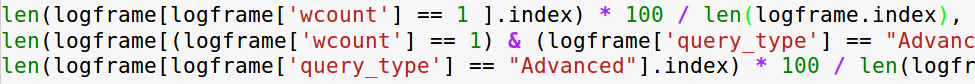
\includegraphics[width=1\textwidth]{pics/erste_Auswertung}
  \end{center}
  96.3 Prozent aller einfachen Suchanfragen beinhalten nur ein Suchwort.\\
  62.7 Prozent aller erweiterten Suchanfragen beinhalten ebenfalls nur ein Suchwort.\\
  8.4 Prozent aller Suchanfragen werden über die erweiterte Suche durchgeführt.
\end{frame}

\only<article>{
  Na, erscheinen uns die Werte plausibel? Hier liegt der Vorteil in den Methoden der DataScience: Erste Auswertungen und Übersichten kosten nichts. So brauchte die Auswertung zu den Suchanfragen über sechs Millionen Zeilen nur knapp drei Sekunden. Zum Vergleich: Das Laden aller Daten ins den DataFrame dauert ca. 30 Sekunden, ein Versuch, dieselben Daten in Excel zu laden bringt die Software zum Absturz. 

  Wir können also jederzeit in die Daten schauen und sie bei jedem Schritt auf Plausibilität überprüfen. Im obigen Beispiel gab es einen Fehler bei der Aufteilung des Strings in Suchworte.
}

\begin{frame}{anonymisierte Logdaten aus dem Discovery--Portal}
  \framesubtitle{2. Auswertung mit DataScience--Methoden}
  Die korrekten Zahlen:
  
  23.86981985807454 Prozent aller einfachen Suchanfragen beinhalten nur ein Suchwort.\\
  26.29683387412833 Prozent aller erweiterten Suchanfragen beinhalten ebenfalls nur ein Suchwort.\\
  8.357088529815087 Prozent aller Suchanfragen werden über die erweiterte Suche durchgeführt.\\
  Die Auswertung dauerte  1.91  Sekunden.
\end{frame}

\only<article>{
  Der Einsatz von DataScience Methoden ist nicht immer optimal. So war es wesentlich einfacher, die 150 Millionen Zeilen mit awk auf die relevanten sechs Millionen einzudampfen, als alle Daten erst in ein Dataframe zu laden und dann die relevanten zu extrahieren.
}

\begin{frame}{DataScience für alles?}
  
  Bsp. Benutzerdatensplitting: Automatisiertes Splitten von 100 Datensätzen, die aus zwei Elementen bestehen, in Vor- und Nachname:
  \medskip

  \begin{tabular}{lrl}
    mit Python und nltk: & 16.73 & Sekunden\tabularnewline
    mit Python ohne nltk: & 0.69 & Sekunden\tabularnewline
    mit Ruby: & 0.39 & Sekunden\tabularnewline
  \end{tabular}
  \medskip

  Das wirkt sich bei 650‘000 Datensätzen schon deutlich aus.
\end{frame}

\begin{frame}{DataScience--Methoden zum Sichten}
  Auch bei ,,wenigen'' Daten können Methoden aus der DataScience genutzt werden, um sich schnell einen Überblick zu verschaffen und danach das weitere Vorgehen aufgrund von Fakten besser planen zu können.
  
\end{frame}
\begin{frame}{DataScience--Methoden zum Sichten}
  Wieder am Beispiel Benutzerdatensplitting: Visualisierung der Ergebnisse einer maschinellen Bearbeitung:
  \begin{center}
    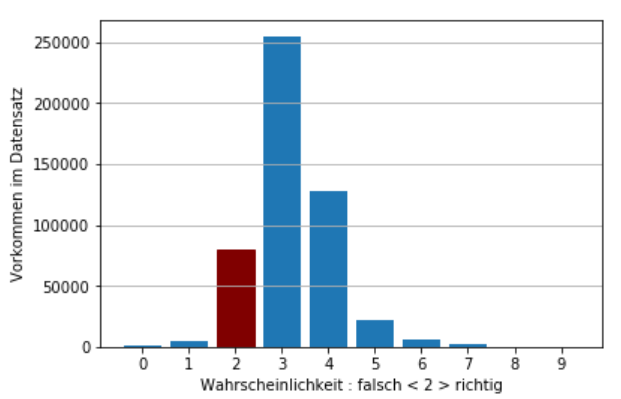
\includegraphics[width=1\textwidth]{pics/Auswertung_Splitting}
  \end{center}
  
\end{frame}


\begin{frame}{BigData Technologien für small data:}
  \framesubtitle{Alter Ansatz mit relationaler DB:}
  Aufbau eines OAI--Servers für die Daten der graphischen Sammlung: 23‘275 Datensätze, annähernd OAI_DC, Veränderung in den letzten Monaten nichtmal ein Datensatz / Woche

  \textbf{gestern:}\\
  Alle Quelldaten werden bereinigt und konvertiert, so dass sie beim Publishen direkt aus der DB gezogen und korrekt ausgegeben werden können.
  \begin{center}
    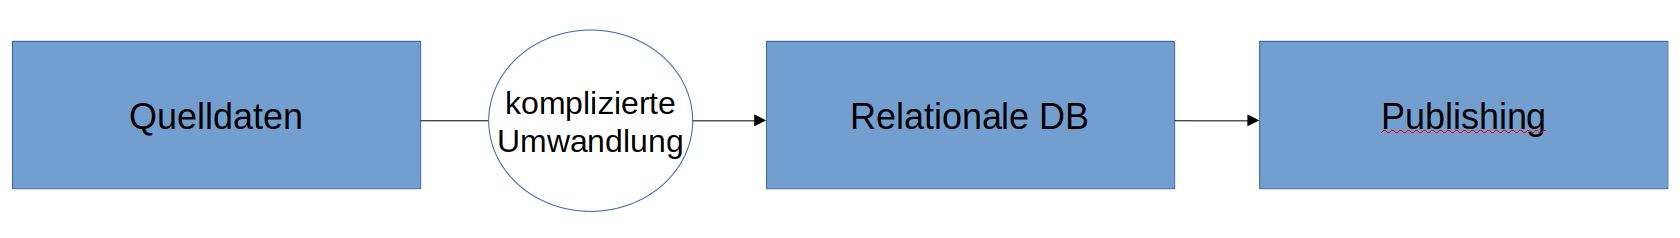
\includegraphics[width=1\textwidth]{pics/Ansatz-mit-rel-DB}
  \end{center}
  
\end{frame}

\begin{frame}{BigData Technologien für small data:}
  \framesubtitle{Neuer Ansatz mit dokumentenorientierter DB:}
  \textbf{heute:}\\
  Alle Quelldaten werden unverändert in eine dokumentenorientierte DB, die gut skalierbar ist, geladen. Die Umwandlung passiert erst beim Publishing. 
  \begin{center}
    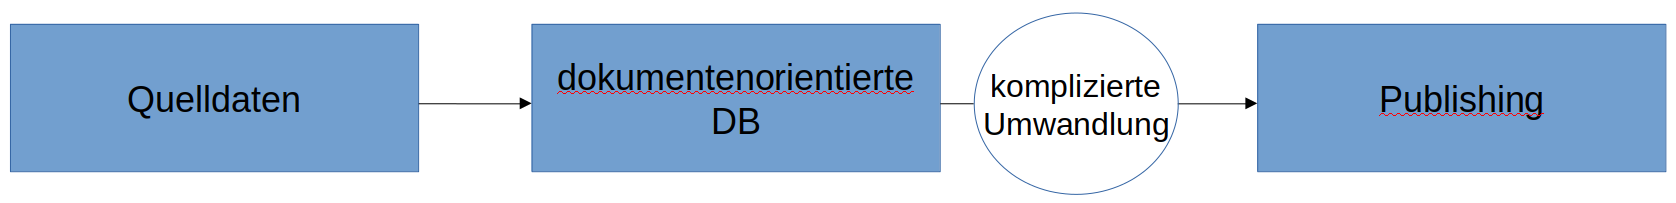
\includegraphics[width=1\textwidth]{pics/Ansatz-mit-dok-DB}
  \end{center}
  
\end{frame}
  
\end{frame}

\begin{frame}{BigData Technologien für small data:}
  \framesubtitle{Neuer Ansatz mit dokumentenorientierter DB:}
  \textbf{morgen:}\\
  Dadurch dass die Umwandlung erst beim Publishing passiert und somit alle Daten komplett und unverändert in der DB vorhanden sind, lassen sich aus den Quelldaten und Verknüpfungen mit weiteren Daten umfangreiche Auswertungen ziehen.
  \begin{center}
    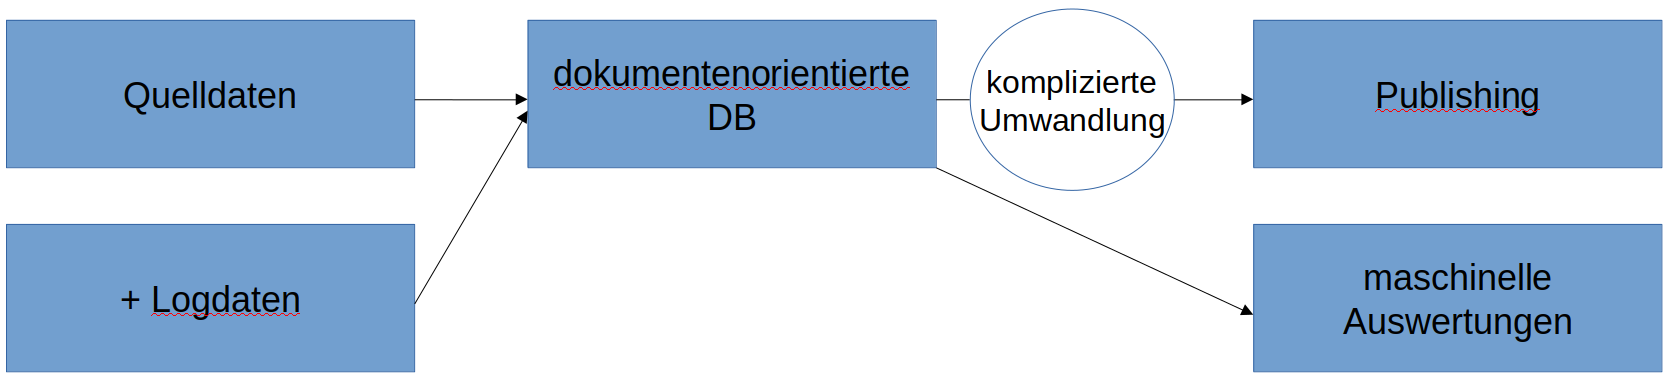
\includegraphics[width=1\textwidth]{pics/zuknft-mglk}
  \end{center}
  
\end{frame}

\section{Von Verschlüsselung via hashing zur BlockChain}
\subsection{Verschlüsselung}
\only<article>{
  Das Problem bei allen Anwendungen im Netz --- seien es Cloud--Applikationen oder einfach nur der Versand einer E--Mail --- ist, dass die Daten auf ihrem Weg mitgelesen werden können. Tatsächlich fliegt eine Mail so offen durch das Netz, wie eine Postkarte vom Urlaubsort zum Empfänger.

  Damit im Postverkehr nicht jeder meine Gedanken verfolgen kann, packe ich sie in einen verschlossenen Umschlag. Mails müsste man verschlüsseln. Das ist jedoch immer noch relativ kompliziert, so dass der meiste E--Mail--Verkehr immer noch offen durch's Netz fliegt.

  Leider hinkt auch sonst der Vergleich mit der guten alten Post: Während im Postwesen unsere Kommunikation in vielen Ländern durch das Fernmeldegeheimnis geschützt ist, nehmen sich die Staaten bei digitaler Kommunikation das Recht, im grossen Stil mitzulesen. 
  
  \begin{quote}
    Was man für sich behalten möchte, gehört nicht ins Netz.
  \end{quote}

  Damit ergibt sich nun ein Problem: Wenn ich etwas verschlüsseln und mit jemand anderem austauschen möchte, müssen wir uns über den Schlüssel verständigen. Das ist Einfach, wenn der Kommunikationspartner nebenan wohnt. Ich gehe einfach rüber und wir bauen uns einen digitalen Schlüssel, mit dem wir unsere Texte zukünftig ver- und wieder entschlüsseln. 

  Jeder, der an unserer Kommunikation teilnehmen möchte, bekommt den Schlüssel und kann von da ab alles Mitlesen.

  Das wird nun schwierig, wenn einer der Partner nicht am selben Ort ist. Man kann sich den erstellten Schlüssel ja schlecht per Mail schicken. Die Mail kann gelesen werden, und jeder, der den Schlüssel hat, kann den gesamten Verkehr entschlüsseln.

  Darum wurde die asymmetrische Verschlüsselung entwickelt. Sie basiert darauf, dass jeder Teilnehmer einen eigenen Schlüssel zum entschlüsseln und einen sogenannten öffentlichen Schlüssel von jedem seiner Kommunikationspartner zum verschlüsseln hat.

  Nochmal: Jeder hat einen privaten Schlüssel, mit dem er die an sich selber gerichtete Kommunikation entschlüsseln kann, und einen öffentlichen Schlüssel, mit dem alle anderen die an ihn gerichtete Kommunikation verschlüsseln können. 

  Der Ablauf ist nun folgender: Ich möchte eine Mail an meinen Freund, nennen wir ihn Hans Heimlich, schicken. Hans Heimlich schickt mir ganz offen seinen öffentlichen Schlüssel. Er liegt auch auf diversen Schlüsselservern, damit jeder, der mit ihm in Kontakt treten möchte, den Schlüsseln finden kann.

  Diesen öffentlichen Schlüssel von Hans Heimlich benutze ich nun, um den an ihn gerichteten Text zu verschlüsseln. Nachdem ich den Text verschlüssetl habe, kann ich ihn selber nicht mehr lesen. Denn mit dem öffentlichen Schlüssel kann man zwar verschlüsseln, aber nicht entschlüsseln! Ich kann also den verschlüsselten Text über das Netz versenden, und niemand kann ihn (mit vertretbarem Aufwand --- bei aktuellen Schlüsseln brauchen Supercomputer Tage bis Wochen, um eine Mail zu entschlüsseln) mitlesen.

  Der verschlüsselte Text kommt also bei Hans Heimlich an. Er nimmt nun seinen \emph{privaten} Schlüssel, um den Text zu entschlüsseln. Sein privater Schlüssel ist der einzige, mit dem man den Text wieder entschlüsseln kann. Deshalb achtet Hans Heimlich darauf, ihn nicht zu verlieren, aber auch darauf, dass er keinesfalls im Netz landet! Also kein Backup des Schlüssels auf DropBox, Google-- oder iCloudDrive!

  Und das macht die Verschlüsselung so sicher wie unpraktisch: Heute lesen wir Mails nicht mehr nur auf einem Gerät. Wir müssten den privaten Schlüssel aber auf jedem Gerät haben, mit dem wir Mails empfangen --- also auch auf dem Smartphone. Keine gute Idee! 

  Praktikable Lösungen für dieses Problem gibt es noch nicht. 
}
\subsection{hashing}
\only<article>{
  Bei Dateien, die wir aus dem Netz laden, seien es öffentliche Schlüssel, Dokumente oder Software, ergibt sich immer die Frage, ob ich auch wirklich die Datei bekommen habe, die ich haben wollte. Das schauen wir uns an einem Beispiel an. 

  Ein Programmierer, Mr. Goodcode unterhält eine Webseite, auf der er seine Software anbietet, die Dokumentation und eine FAQ--Seite pflegt. Die Software kann man sich herunter laden. Da für  Webseiten die Datenmenge, die herauf und herunter geladen werden kann üblicherweise begrenztund teuer ist, liegt die Software nicht in einem Unterverzeichnis der Webseite, sondern bei einem File--Hoster. Der Benutzer wird also bei Klick auf den Download--Link auf die Seite des File--Hosters weiter geleitet, von wo aus der Download dann direkt startet.

  Nun wechseln wir mal die Perspektive und schlüpfen in die Rolle des Hackers Mr. Badcode. Badcode hat einen Schadcode entwickelt und möchte ihn auf möglichst viele Rechner verteilen. Er hackt sich in die Server eines File--Hosters ein, entpackt die dort liegenden Downloads, fügt den Programmen seinen Schadcode hinzu und verpackt alles wieder. Niemand bemerkt seinen Einbruch und ab sofort lädt jeder, der von dem Filehoster Software bezieht, den Schadcode von Badcode mit aif seinen PC.

  Mr. Goodcode möchte das verhindern und sicherstellen, dass die Kunden seine Software unverändert bekommen, wenn sie sie irgendwo aus dem Netz herunter laden. Glücklicherweise gibt es eine Lösung: Mr. Goodcode berechnet auf seinem Computer von seiner Software mit einem weit verbreiteten Algorithmus eine Prüfsumme, einen sogenannten hash. 

  Ein hash ist vergleichbar mit einer Quersumme einer Zahl. Allerdings wird durch den Algorithmus sichergestellt, dass mit einer sehr grossen Wahrscheinlichkeit keine zwei unterschiedlichen Codes die gleiche Prüfsumme ergeben können.

  Mr. Goodcode verteilt nun seine Software im Netz und veröffentlicht auf seiner Webseite die Prüfsumme. Wer sich jetzt die Software irgendwo herunter lädt, erzeugt von dem erhaltenen Download mit dem gleichen Algorithmus die Prüfsumme und vergelicht sie mit der auf der Webseite veröffentlichten. Stimmt sie überein, ist die Software unverändert. Mr. Badcode müsste sich nun in den File--Hoster und zusätzlich in die Webseite von Mr. Goodcode hacken, um sowohl den Download als auch den veröffentlichten hash zu manipulieren. Und diese Manipulation auf seiner Webseite würde Mr. Goodcode schnell auffallen.
}

\subsection{BlockChain}
\only<article>{
  In der ersten Lektion hatten wir uns ein Konzept angesehen, mit dem man wachsenden Datenmengen begegnet: verschiedene Techniken um Daten in mehreren Speichersystemen --- Festplatten oder Datenbanken --- gleichzeitig abzulegen. Das Problem dabei ist, sicher zu stellen, dass die Daten in allen Speichern konsistent sind. Sie zu vergleichen würde viel zu viel Rechenzeit kosten. Stattdessen hasht man sie (bzw. Teile davon) und vergleicht die hashes. Dafür braucht es aber einen ,,Master'', der die Transaktionen überwacht und die Verantwortung dafür übernimmt, dass alle Daten über alle Systeme einen konsistenten Zustand haben. Mit diesem Master haben wir aber auch wieder einen Single Point of Failure --- fällt er aus, ist das ganze System unbrauchbar.

  Mit der BlockChain wird dieses Problem gelöst. Hier sind alle Geräte gleichberechtigt dafür verantwortlich, dass alle denselben Stand haben. Eine einfache Mehrheit genügt, um zu bestätigen, dass eine Transaktion so gelaufen ist, wie die gelaufen ist. Oder umgekehrt: Um eine Transaktion zu fälschen, muss man 51\% aller Ressourcen unter seine Kontrolle bringen.

  Dazu kommt ein weiteres Konzept: Die Transaktionen werden in Blöcke zusammengefasst. Dann wird über den Block ein hash gebildet. Über diesem hash und dem hash der vorangegangenen Blocks wird ein weiterer hash gebildet, der wieder im nächsten Block abgelegt wird. So würde das Fälschen einer Transaktion alle folgenden ungültig machen.

  \begin{center}
     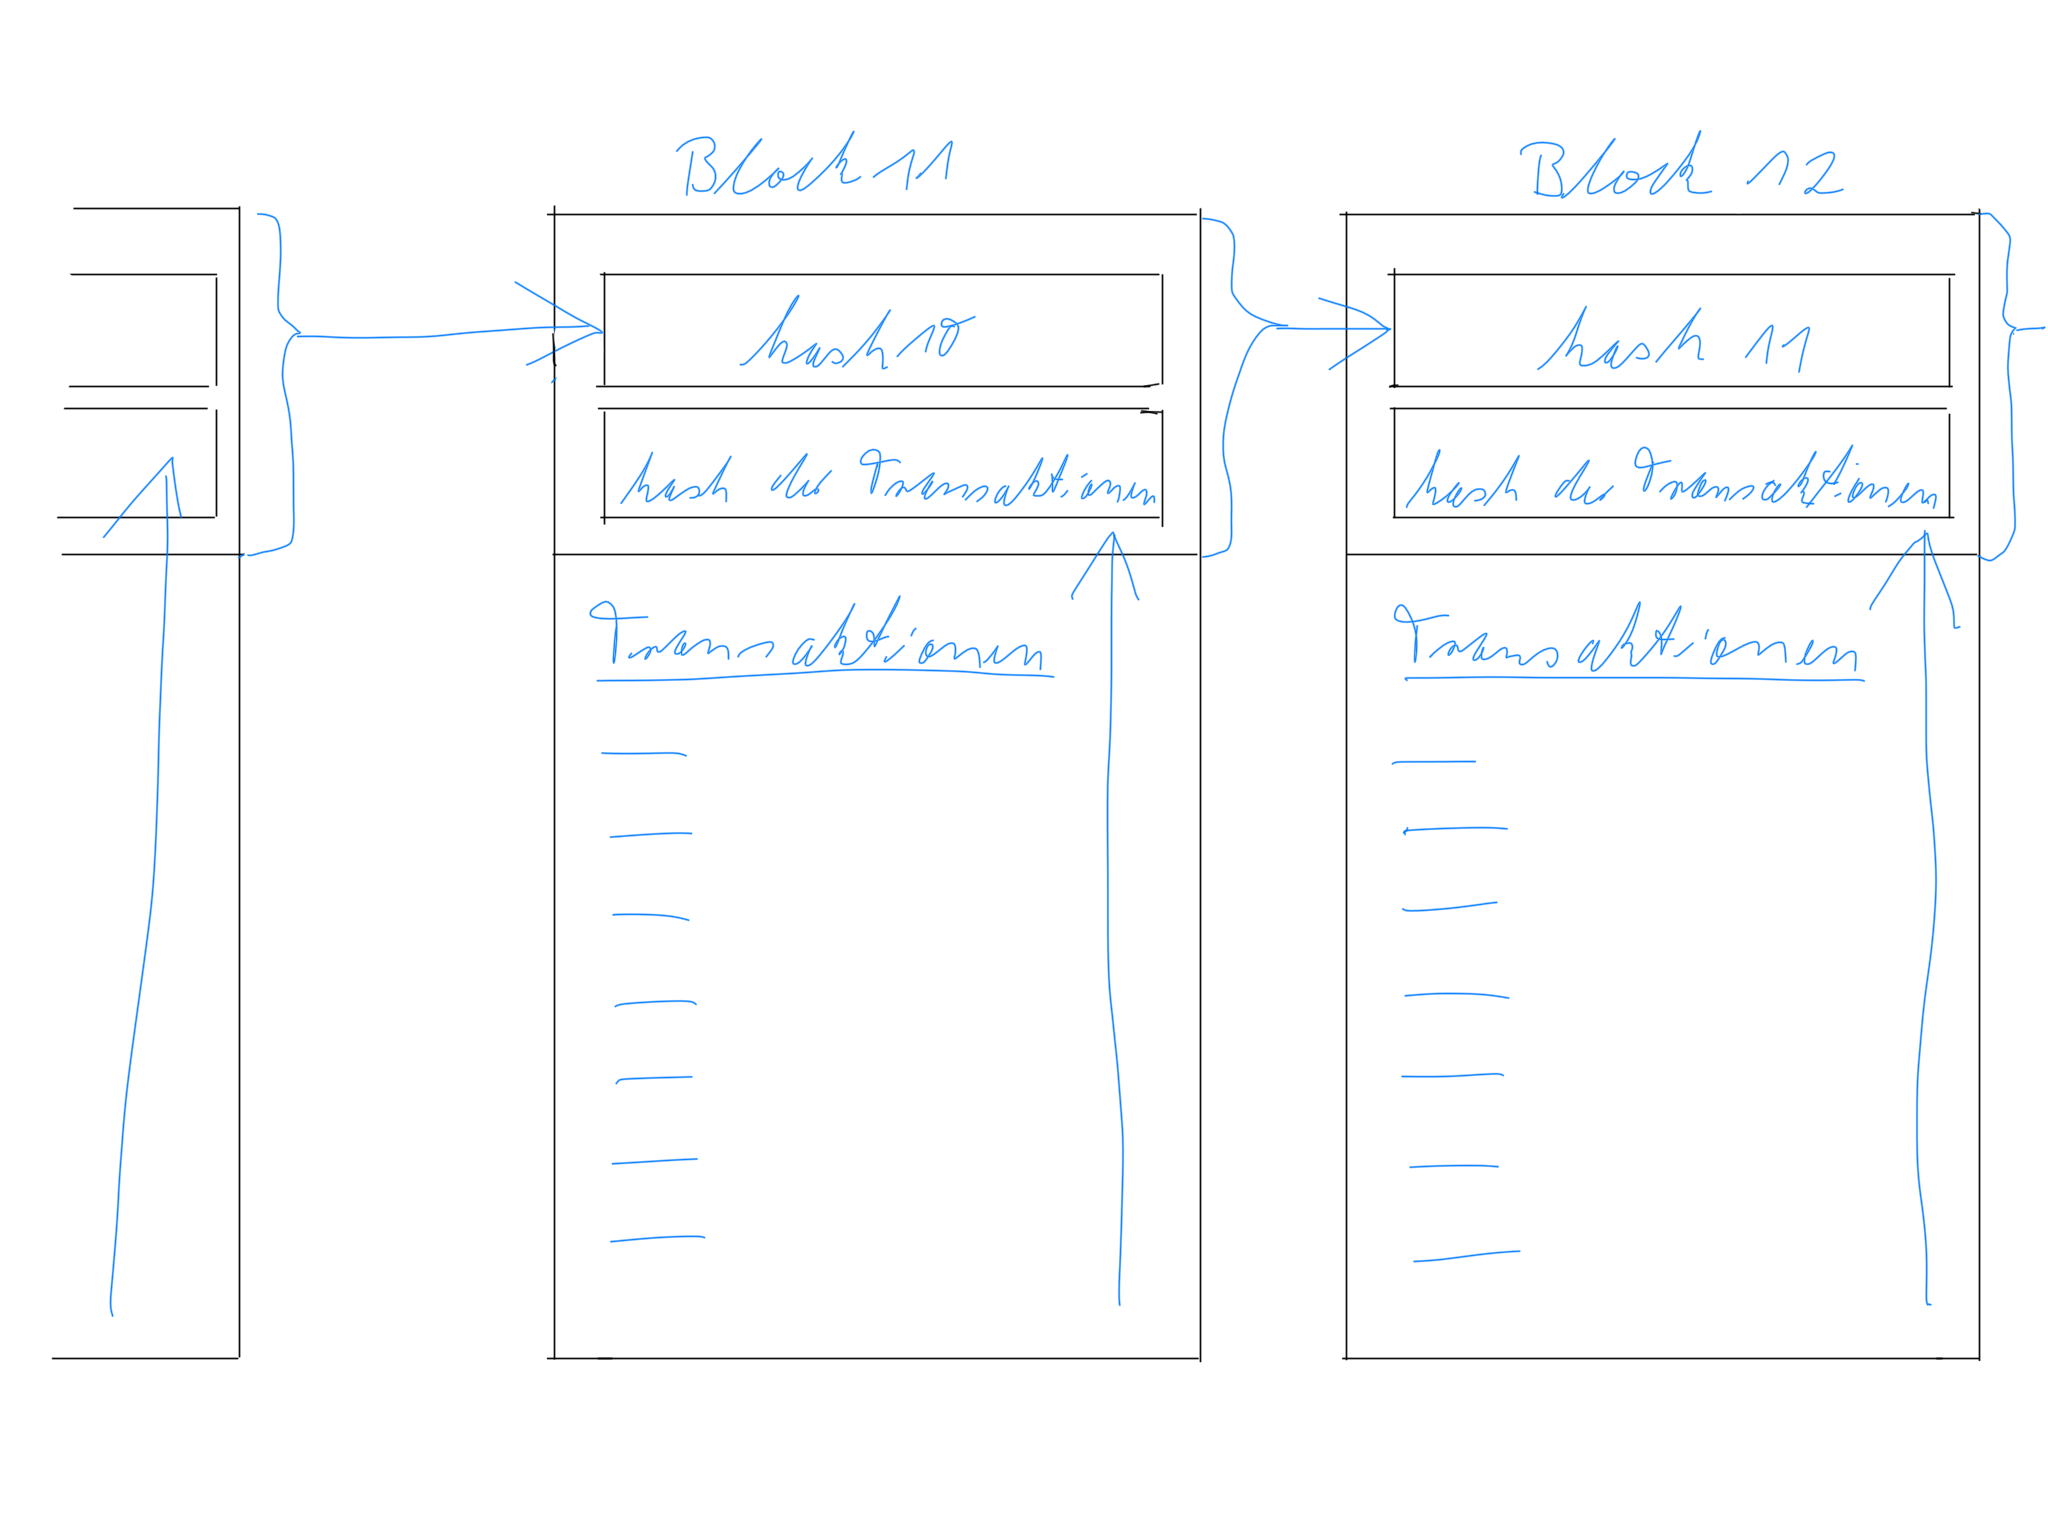
\includegraphics[width=1\textwidth]{pics/bitcoin}
   \end{center}

  Das Konzept hat natürlich auch Nachteile: Zum einen liegen immer alle Daten auf allen Systemen redundant vor. Bitcoin beispielsweise belegte im Januar 2018 rund 150 GB auf der Platte, und das redundant auf jedem teilnehmenden System. Zum anderen wird das Berechnen der hashes immer aufwendiger, je länger die Kette wird. Der Energiehunger von BitCoin liegt laut des \href{https://digiconomist.net/bitcoin-energy-consumption}{Bitcoin Energy Consumption Index} bei rd. 50 TWh, das entspricht dem Strombedarf von Portugal. 

  Und gerade bezüglich digitaler Währungen gibt es ein nicht zu unterschätzendes Risiko: Die Sicherheit der Transaktionen beruht auf der Annahme, dass ein einzelner nicht genügend Rechenleistung zur Verfügung hat, um die Hashes zu knacken und Manipulationen schneller vornehmen zu können, als alle anderen benötigen, die Kette weiter zu verlängern. Es ist inzwischen recht wahrscheinlich, dass Quantencomputer in absehbarer Zeit Realität werden. Der erste Quantencomputer währe so schnell, dass er die Blockchain aushebeln könnte. Wenn sich bis dahin das Konzept nicht noch weiter optimiert haben wird, wäre die Währung auf einen Schlag wertlos.
}
